% !TeX root = ../thesis.tex

\section{Results}

\subsection{RQ1: Probability of failure}\label{ssec:results-rq1}
The two pie charts in \Cref{fig:rq1-failure-probability} illustrate the amount of failed and successful test runs. The leftmost chart visualises the failure rate in the dataset \cite{travisanalysis} by Durieux et al. $\SI{4558279}{}$ test runs out of the $\SI{28882003}{}$ total runs have failed, which corresponds to a failure probability of $\SI{18.74}{\percent}$. The other pie chart uses data from the TravisTorrent \cite{msr17challenge} project. Since we can infer the cause of failure from this dataset, it is possible to obtain more accurate results. $\SI{42.89}{\percent}$ of the failed runs are due to a compilation failure where the test suite did not execute. For the remaining part of the runs, $\SI{225766}{}$ out of $\SI{2114920}{}$ executions contain at least one failed test case, corresponding to a failure percentage of $\SI{10.67}{\percent}$.

\begin{figure}[htbp!]
	\centering
	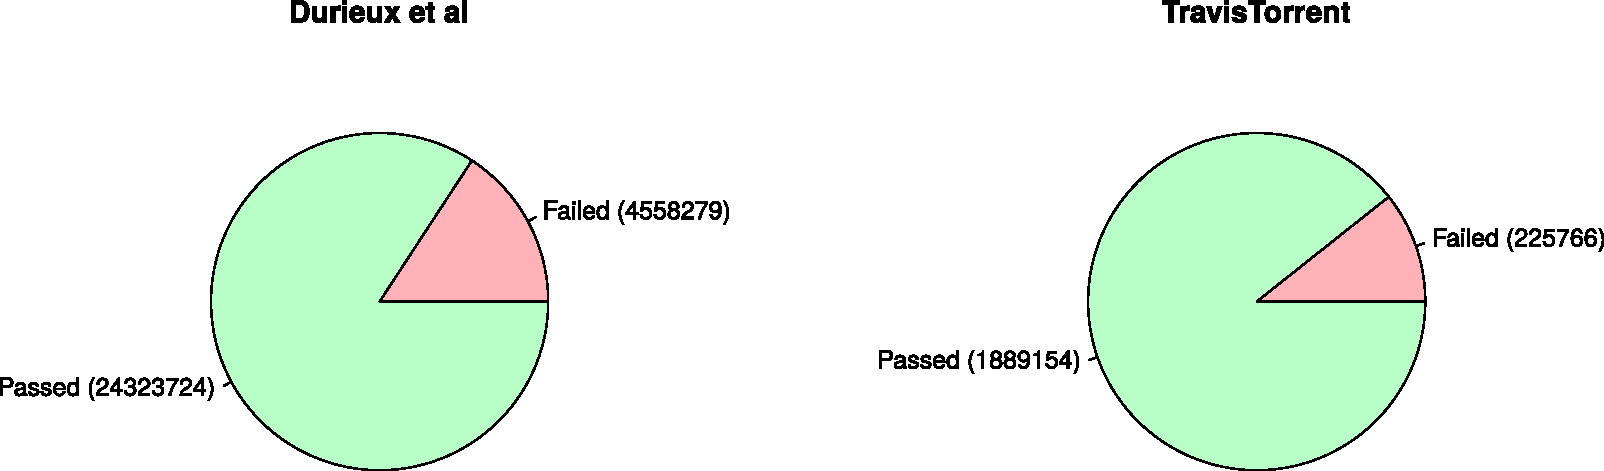
\includegraphics[width=\textwidth]{assets/charts/rq1-failure-probability.pdf}
	\caption{Probability of test run failure.}
	\label{fig:rq1-failure-probability}
\end{figure}

\subsection{RQ2: Average duration of a test run}
The dataset by Durieux et al. \cite{travisanalysis} has been refined to only include test runs that did not finish within $\SI{10}{s}$. A lower execution time generally indicates that the test suite did not execute and that a compilation failure has occurred instead. \Cref{tbl:rq2-characteristics} contains the characteristics of the remaining $\SI{24320504}{}$ analysed test runs. The median and average execution times suggest that primarily small projects are \travisci{}, yet the maximum value is very high. \Cref{fig:rq2-durations} confirms that $\SI{71378}{}$ test runs have taken longer than one hour to execute. Further investigation has revealed that these are typically projects which are using mutation testing, such as \texttt{plexus/yaks}\footnote{A Ruby library for hypermedia (\url{https://github.com/plexus/yaks}).}.

\begin{table}[h]
	\centering
	\begin{tabularx}{\textwidth}{|C|C|C|C|C|}
		\hline
		\textbf{\# runs} & \textbf{Minimum} & \textbf{Mean} & \textbf{Median} & \textbf{Maximum}\\
		\hline
		$\SI{24320504}{}$ & $\SI{10}{\second}$ & $\SI{385}{\second}$ & $\SI{178}{\second}$ & $\SI{26}{\hour} \SI{11}{\minute} \SI{26}{\second}$\\
		\hline
	\end{tabularx}
	\caption{Characteristics of the test run durations in \cite{travisanalysis}.}
	\label{tbl:rq2-characteristics}
\end{table}

\begin{figure}[htbp!]
	\centering
	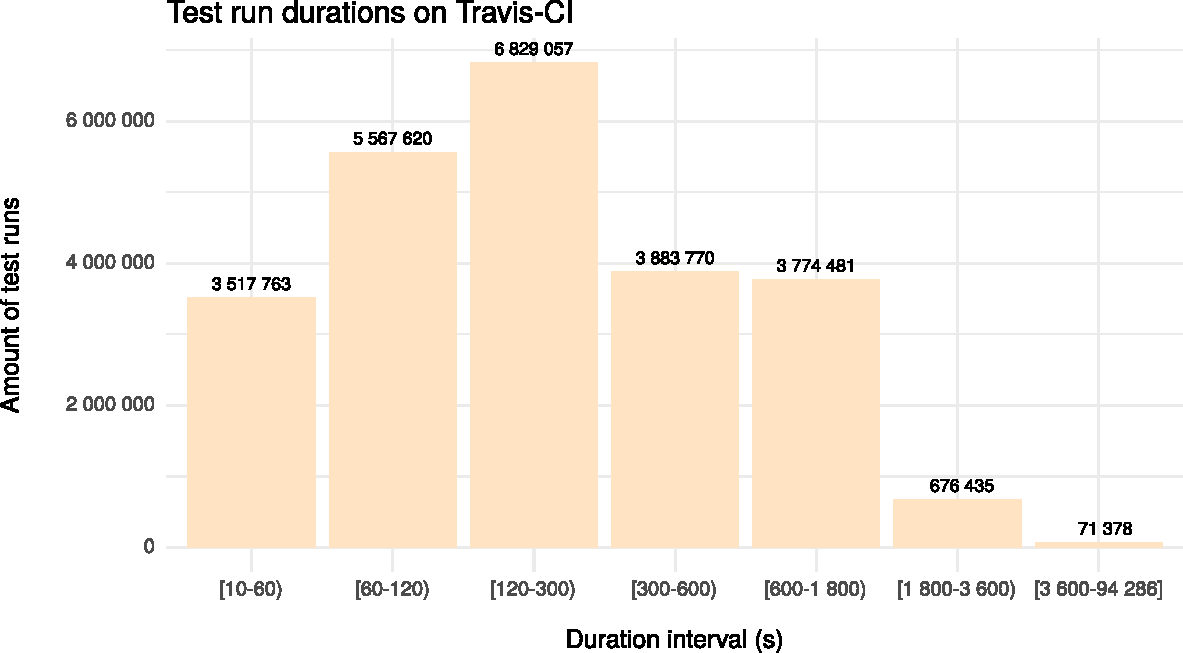
\includegraphics[width=\textwidth]{assets/charts/rq2-test-run-durations.pdf}
	\caption{Test run durations on \travisci{}.}
	\label{fig:rq2-durations}
\end{figure}


\subsection{RQ3: Consecutive failure probability}
Because the TravisTorrent project is the only dataset that contains the identifier of the previous run, only runs from this project have been used. This dataset consists of $\SI{211040}{}$ test runs, immediately following a failed execution. As illustrated in \Cref{fig:rq3-consecutive-failure}, $\SI{109224}{}$ of these test runs have failed as well, versus $\SI{101816}{}$ successful test runs ($\SI{51.76}{\percent}$).

\begin{figure}[htbp!]
	\centering
	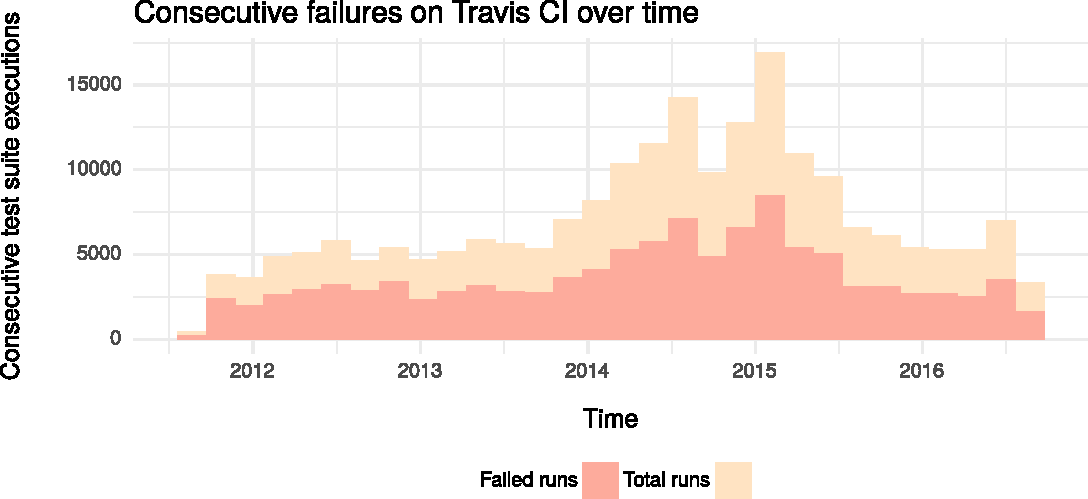
\includegraphics[width=\textwidth]{assets/charts/rq3-consecutive-failure.pdf}
	\caption{Consecutive test run failures on \travisci{}.}
	\label{fig:rq3-consecutive-failure}
\end{figure}

\subsection{RQ4: Applying \tcp{} to Dodona}
After executing the $\SI{120}{}$ failed test runs, the log files have been inspected. These log files have revealed that an error in the configuration was the actual culprit of five failed test runs, rather than a failed test case. These test runs have therefore been omitted from the results because the test suite did not execute. Since configuration-related problems require in-depth contextual information about the project, we cannot automatically predict these.\\

\noindent \Cref{tbl:rq4-first-failure} contains the amount of executed test cases until we observe the first failure. These results indicate that every predictor is capable of performing at least one successful prediction. Furthermore, the maximum amount of executed test cases is lower than the original value, which means that every algorithm is a valid predictor. The data suggests that the Alpha algorithm and the HGS algorithm are the preferred predictors for the Dodona project. In contrast, the performance of the ROCKET algorithm is rather low.\\

\begin{table}[h]
	\centering
	\begin{tabularx}{\textwidth}{|X||c|c|c|c|}
		\hline
		\textbf{Algorithm} & \textbf{Minimum} & \textbf{Mean} & \textbf{Median} & \textbf{Maximum}\\
		
		\hline
		
		\emph{Original} & $\SI{0}{}$ & $\SI{155}{}$ & $\SI{78}{}$ & $\SI{563}{}$\\
		
		\hline
		
		Alpha & $\SI{0}{}$ & $\SI{8}{}$ & $\SI{3}{}$ & $\SI{73}{}$\\
		
		\hline
		AffectedRandom & $\SI{0}{}$ & $\SI{54}{}$ & $\SI{10}{}$ & $\SI{428}{}$\\
		AllInOrder & $\SI{0}{}$ & $\SI{119}{}$ & $\SI{82}{}$ & $\SI{460}{}$\\
		AllRandom & $\SI{0}{}$ & $\SI{90}{}$ & $\SI{27}{}$ & $\SI{473}{}$\\
		
		\hline
		
		GreedyCoverAffected & $\SI{0}{}$ & $\SI{227}{}$ & $\SI{246}{}$ & $\SI{494}{}$\\
		GreedyCoverAll & $\SI{0}{}$ & $\SI{98}{}$ & $\SI{33}{}$ & $\SI{514}{}$\\
		GreedyTimeAll & $\SI{0}{}$ & $\SI{210}{}$ & $\SI{172}{}$ & $\SI{482}{}$\\
		
		\hline
		
		HGSAffected & $\SI{0}{}$ & $\SI{61}{}$ & $\SI{10}{}$ & $\SI{511}{}$\\
		HGSAll & $\SI{0}{}$ & $\SI{124}{}$ & $\SI{54}{}$ & $\SI{507}{}$\\
		
		\hline
		
		ROCKET & $\SI{0}{}$ & $\SI{210}{}$ & $\SI{170}{}$ & $\SI{482}{}$\\
		
		\hline
	\end{tabularx}
	\caption{Amount of executed test cases until the first failure.}
	\label{tbl:rq4-first-failure}
\end{table}

\noindent The previous results have been visualised in \Cref{fig:rq4-performance}. These charts confirm the low accuracy of the ROCKET algorithm. The Alpha algorithm and the HGS algorithm offer the most accurate predictions, with the former algorithm being the most consistent. Observe the chart of the Greedy algorithm. This algorithm manages to very accurately predict some of the test runs while failing to predict others anywhere near, a behaviour which is specific to a greedy heuristic.\\

\clearpage

\begin{figure}[!hbp]
	\subfloat[Alpha algorithm]{%
		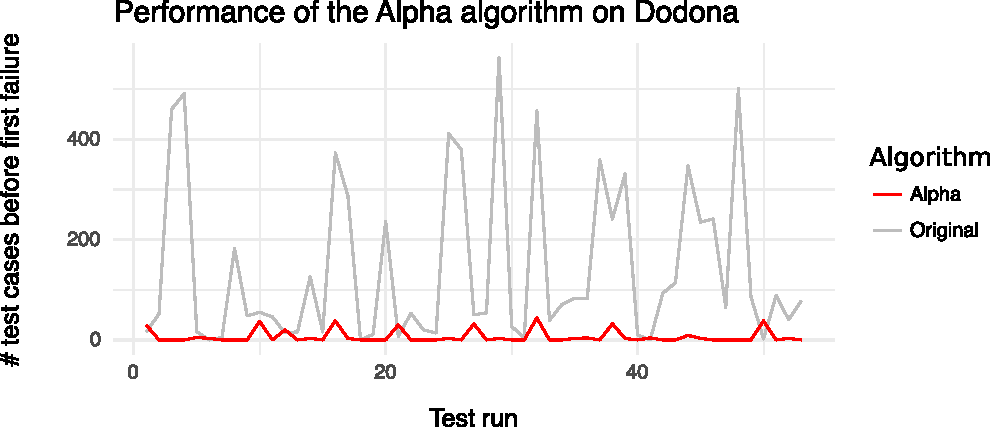
\includegraphics[width=\textwidth]{assets/charts/rq4-dodona-alpha.pdf}
	}
	\phantomcaption
\end{figure}
\begin{figure}[!hbp]
	\ContinuedFloat
	\subfloat[Greedy algorithm]{%
		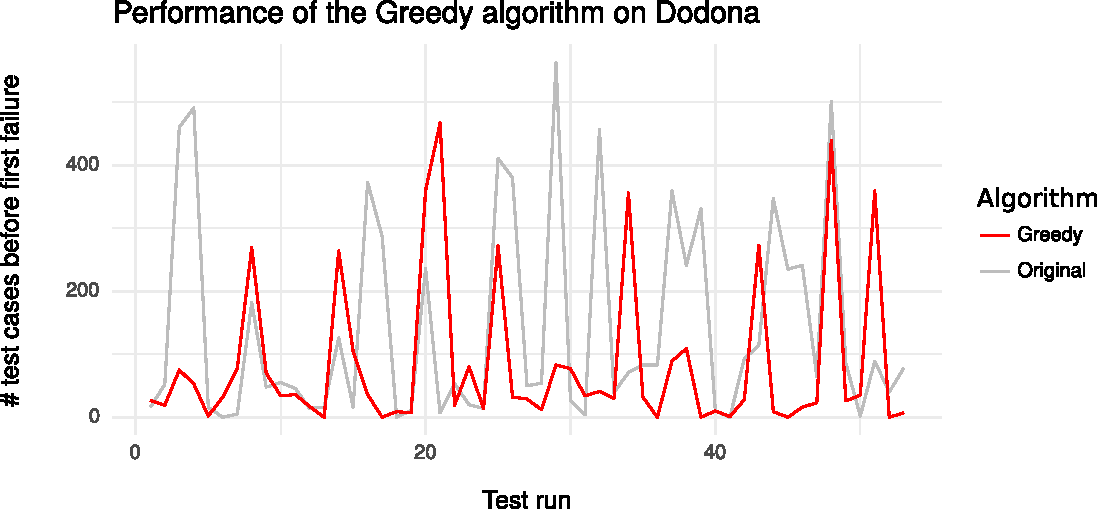
\includegraphics[width=\textwidth]{assets/charts/rq4-dodona-greedy.pdf}
	}
	\phantomcaption
\end{figure}
\begin{figure}[!hbp]
	\ContinuedFloat
	\subfloat[HGS algorithm]{%
		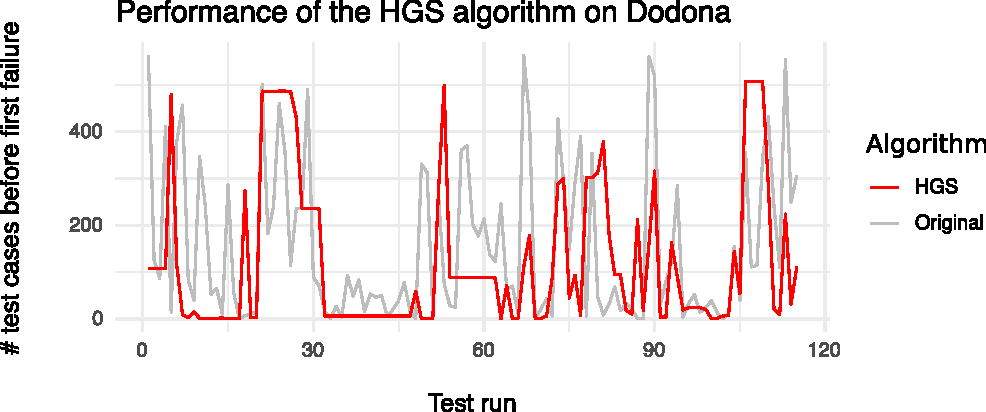
\includegraphics[width=\textwidth]{assets/charts/rq4-dodona-hgs.pdf}
	}
	\phantomcaption
\end{figure}
\begin{figure}[!t]
	\ContinuedFloat
	\centering
	\subfloat[ROCKET algorithm]{%
		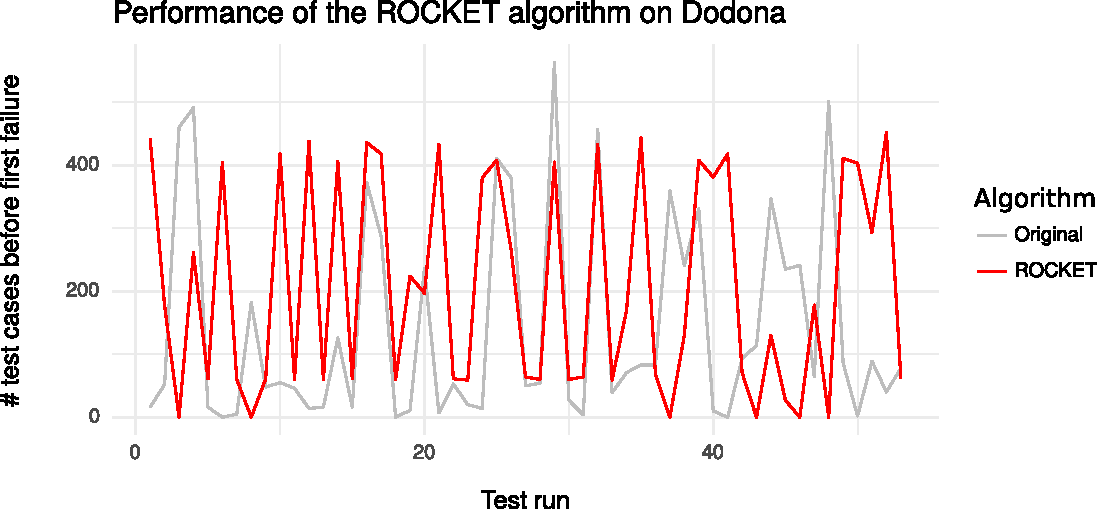
\includegraphics[width=\textwidth]{assets/charts/rq4-dodona-rocket.pdf}
	}
	\caption{Prediction performance on the Dodona project.}
	\label{fig:rq4-performance}
\end{figure}

\noindent The duration until the first observed failure is reported in \Cref{tbl:rq4-first-failure-duration}. Observe that the previous table indicates that the ROCKET algorithm does not perform well, while this table suggests otherwise. We can explain this behaviour by examining the objective function of this algorithm. This function prioritises cases with a low execution time to be executed first.\\

\begin{table}[htbp!]
	\centering
	\begin{tabularx}{\textwidth}{|X||c|c|c|c|}
		\hline
		\textbf{Algorithm} & \textbf{Minimum} & \textbf{Mean} & \textbf{Median} & \textbf{Maximum}\\
		
		\hline
		
		\emph{Original} & $\SI{0}{\second}$ & $\SI{135}{\second}$ & $\SI{123}{\second}$ & $\SI{380}{\second}$\\
		
		\hline
		
		Alpha & $\SI{0}{\second}$ & $\SI{3}{\second}$ & $\SI{1}{\second}$ & $\SI{33}{\second}$\\
		
		\hline
		AffectedRandom & $\SI{0}{\second}$ & $\SI{28}{\second}$ & $\SI{5}{\second}$ & $\SI{190}{\second}$\\
		AllInOrder & $\SI{0}{\second}$ & $\SI{82}{\second}$ & $\SI{71}{\second}$ & $\SI{270}{\second}$\\
		AllRandom & $\SI{0}{\second}$ & $\SI{43}{\second}$ & $\SI{11}{\second}$ & $\SI{270}{\second}$\\
		
		\hline
		
		GreedyCoverAffected & $\SI{0}{\second}$ & $\SI{88}{\second}$ & $\SI{86}{\second}$ & $\SI{314}{\second}$\\
		GreedyCoverAll & $\SI{0}{\second}$ & $\SI{46}{\second}$ & $\SI{12}{\second}$ & $\SI{280}{\second}$\\
		GreedyTimeAll & $\SI{0}{\second}$ & $\SI{55}{\second}$ & $\SI{32}{\second}$ & $\SI{175}{\second}$\\
		
		\hline
		
		HGSAffected & $\SI{0}{\second}$ & $\SI{35}{\second}$ & $\SI{6}{\second}$ & $\SI{356}{\second}$\\
		HGSAll & $\SI{0}{\second}$ & $\SI{75}{\second}$ & $\SI{34}{\second}$ & $\SI{377}{\second}$\\
		
		\hline
		
		ROCKET & $\SI{0}{\second}$ & $\SI{54}{\second}$ & $\SI{32}{\second}$ & $\SI{175}{\second}$\\
		
		\hline
	\end{tabularx}
	\caption{Duration until the first failure for the Dodona project.}
	\label{tbl:rq4-first-failure-duration}
\end{table}

\clearpage

\subsection{RQ5: Integrate \velocity{} with Stratego}
The data collection phase has already proven that the Java agent is compatible with Stratego. Since \velocity{} is not yet able to predict test cases which have been added in the current commit, we can only use $\SI{35}{}$ of the $\SI{54}{}$ failed test runs.\\

\noindent Similar to the previous test subject, \Cref{tbl:rq5-first-failure} lists how many test cases have been executed before the first observed failure. The table only considers the four main algorithms, since the actual prediction performance was only secondary to this research question, and we have only analysed a small number of test runs. The results suggest that every algorithm except the ROCKET achieves a high prediction accuracy on this project.\\

\begin{table}[h]
	\centering
	\begin{tabularx}{\textwidth}{|X||c|c|c|c|}
		\hline
		\textbf{Algorithm} & \textbf{Minimum} & \textbf{Mean} & \textbf{Median} & \textbf{Maximum}\\
		
		\hline
		
		\emph{Original} & $\SI{0}{}$ & $\SI{68}{}$ & $\SI{2}{}$ & $\SI{278}{}$\\
		
		\hline
		
		Alpha & $\SI{0}{}$ & $\SI{10}{}$ & $\SI{2}{}$ & $\SI{57}{}$\\
		
		\hline
		
		GreedyCoverAll & $\SI{0}{}$ & $\SI{11}{}$ & $\SI{3}{}$ & $\SI{57}{}$\\
		
		\hline
		
		HGSAll & $\SI{0}{}$ & $\SI{9}{}$ & $\SI{4}{}$ & $\SI{50}{}$\\
		
		\hline
		
		ROCKET & $\SI{0}{}$ & $\SI{42}{}$ & $\SI{27}{}$ & $\SI{216}{}$\\
		
		\hline
	\end{tabularx}
	\caption{Amount of executed test cases until the first failure.}
	\label{tbl:rq5-first-failure}
\end{table}

\noindent Even though the performance of the ROCKET algorithm is suboptimal in the previous table, \Cref{tbl:rq5-first-failure-duration} does indicate that it outperforms every other algorithm time-wise. Notice that the predicted sequence of the HGS algorithm takes the longest to execute, while the previous table suggested a good prediction accuracy. The Alpha and Greedy algorithms seem very similar on both the amount of executed test cases, as well as the execution time. \\

\begin{table}[h]
	\centering
	\begin{tabularx}{\textwidth}{|X||c|c|c|c|}
		\hline
		\textbf{Algorithm} & \textbf{Minimum} & \textbf{Mean} & \textbf{Median} & \textbf{Maximum}\\
		
		\hline
		
		\emph{Original} & $\SI{0}{\second}$ & $\SI{62}{\second}$ & $\SI{8}{\second}$ & $\SI{233}{\second}$\\

		\hline
		
		Alpha & $\SI{0}{\second}$ & $\SI{11}{\second}$ & $\SI{2}{\second}$ & $\SI{103}{\second}$\\
		
		\hline
		
		GreedyCoverAll & $\SI{0}{\second}$ & $\SI{12}{\second}$ & $\SI{2}{\second}$ & $\SI{103}{\second}$\\
		
		\hline
		
		HGSAll & $\SI{0}{\second}$ & $\SI{19}{\second}$ & $\SI{1}{\second}$ & $\SI{130}{\second}$\\
		
		\hline
		
		ROCKET & $\SI{0}{\second}$ & $\SI{6}{\second}$ & $\SI{0}{\second}$ & $\SI{85}{\second}$\\
		
		\hline
	\end{tabularx}
	\caption{Amount of executed test cases until the first failure.}
	\label{tbl:rq5-first-failure-duration}
\end{table}

\noindent \Cref{fig:rq5-performance} further confirms the above statements. Notice the close resemblance of the charts of the Greedy algorithm and the Alpha algorithm, which indicates that a different failing test case is the cause of every test run failure. The ROCKET algorithm performs better on this project than on Dodona, yet not accurate.

\begin{figure}[!hbp]
	\subfloat[Alpha algorithm]{%
		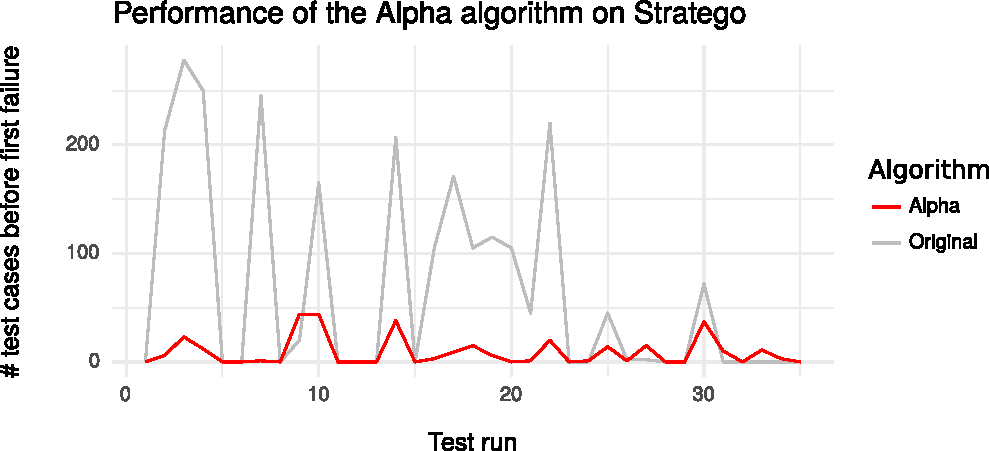
\includegraphics[width=\textwidth]{assets/charts/rq5-stratego-alpha.pdf}
	}
	\phantomcaption
\end{figure}
\begin{figure}[!hbp]
	\ContinuedFloat
	\subfloat[Greedy algorithm]{%
		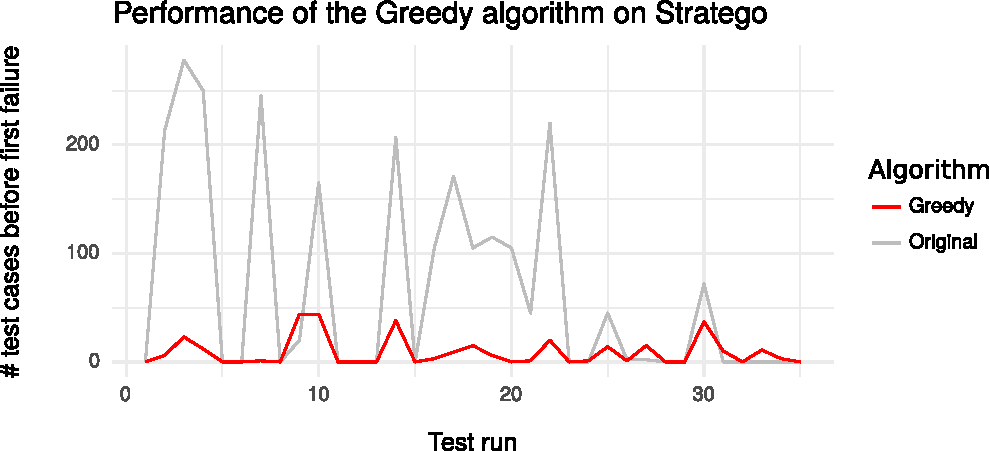
\includegraphics[width=\textwidth]{assets/charts/rq5-stratego-greedy.pdf}
	}
	\phantomcaption
\end{figure}
\begin{figure}[!hbp]
	\ContinuedFloat
	\subfloat[HGS algorithm]{%
		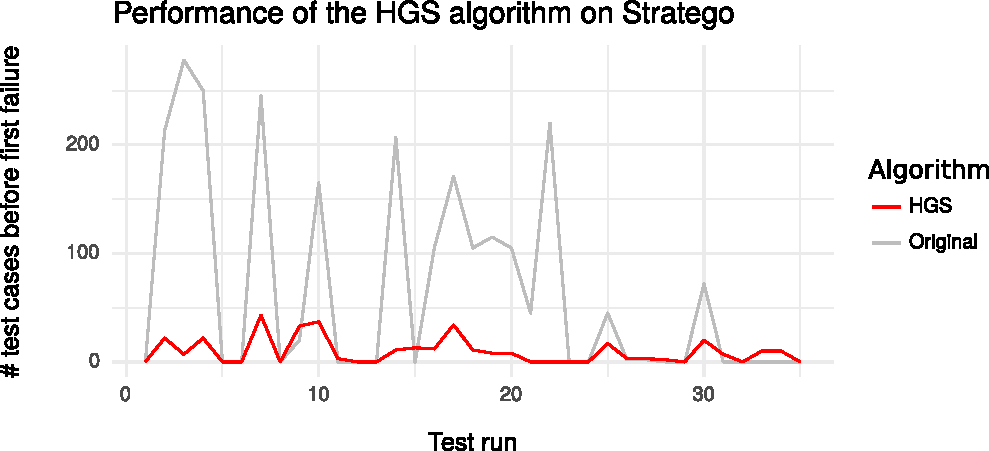
\includegraphics[width=\textwidth]{assets/charts/rq5-stratego-hgs.pdf}
	}
	\phantomcaption
\end{figure}
\begin{figure}[!hbp]
	\ContinuedFloat
	\centering
	\subfloat[ROCKET algorithm]{%
		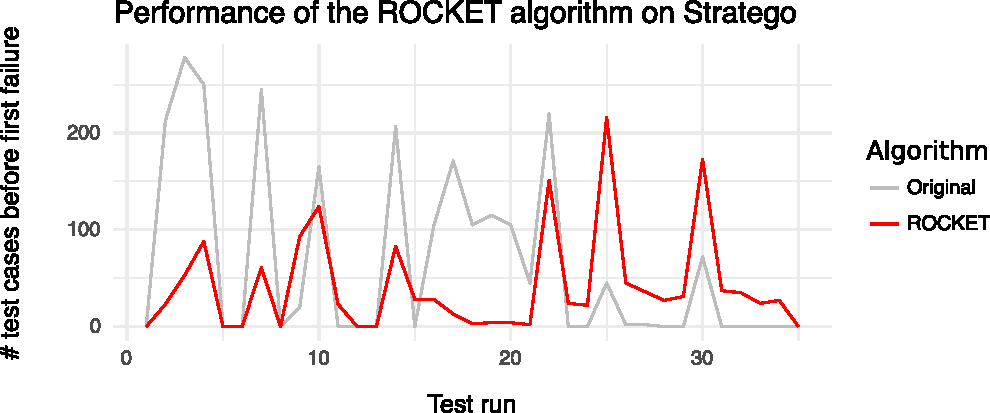
\includegraphics[width=\textwidth]{assets/charts/rq5-stratego-rocket.pdf}
	}
	\caption{Prediction performance on the Stratego project.}
	\label{fig:rq5-performance}
\end{figure}
